\documentclass{article}
\usepackage{epsfig}
\usepackage{hyperref}
\usepackage[margin=0.75in]{geometry}
\usepackage{float}
\usepackage{amsmath}
\usepackage{caption}
\usepackage{subcaption}
\usepackage{algorithm}
\usepackage[noend]{algpseudocode}
\usepackage{afterpage}

\renewcommand{\refname}{\centerline{References}}
\usepackage[numbers]{natbib}
\usepackage{graphicx}

\begin{document}
\pagestyle{empty}
\begin{center}
{\Large{\bf Unsupervised Learning of Religious Facial Features}}\\*[3mm]
{\bf Christopher E. Mertin} \\*[3mm]
\end{center}

\abstract{A paper published by N.O. Rule, {\em et. al}, explored the possibility of humans being able to discern if someone was part of a relgious group or not \cite{MormonID}, and was able to achieve 55\% accuracy. This paper explores the use of unsupervised learning techniques and eigenfaces to perform the same task, with the clustering algorithms obtaining up to 59.3\% labeling accuracy on the clusters, and eigenfaces obtaining upwards of 80\% accuracy on unseen data. }

\section*{Introduction}

A paper by N.O. Rule, {\em et. al}, explored the possibility of being able to identify someone by their religious affiliation based on facial features \cite{MormonID}. In the aforementioned study, a group of volunteers were given photos of people who had Mormon heritage and those who didn't, in an attempt to see if the volunteers could separate them into two groups. The results were that, on average, a person was able to identify who was Mormon or not with 55\% accuracy, which was enough to be statistically significant, though not reliable.

For this project, we explored the use of unsupervised learning techniques to see if these methods can perform at the same level, or better than humans in the study.

In order to obtain photos of these two groups, the Tinder API package Pynder \cite{pynder} was used. To make things simple, only female faces were looked at, though the same techniques can be used for their male counterparts. In order to differentiate from the groups, a users profile was downloaded if their profile said ``LDS,'' or if they went to Bringham Young University. While this isn't 100\% accurate, it does have an accuracy of more than 98\% \cite{byu}, and those false positives are considered noise in the data.

To get faces that were not considered Mormon, not only was the opposite used, but the location was changed to various major cities around the United States. These cities included Seattle, Miami, Los Angeles, New York, Denver, Dallas, Las Vegas, and Raleigh. This was chosen as Mormons are a small percentage of the population, and there is less likely to be a false positive outside of Utah in a city with a large population.

\section*{Transforming Data}

The major difference between the data used in \cite{MormonID} and the data that was used with this project is that the images used in \cite{MormonID} were all taken at the same position. For accuracy, the algorithms used in this project also require the same, so we had to transform the data. 

In order to do so, first a {\em similarity transform} had to be performed on the image. After cropping the faces into individual images, the faces had to be transformed so that they took up a similar coordinate system. The similarity transform can be defined by moving a point from the position $(x,y)$ to the position $(x^{\star}, y^{\star})$ by the equation

\begin{align*}
  \begin{pmatrix}
    x^{\star} \\
    y^{\star}
\end{pmatrix} &= \begin{pmatrix}
\phi_{x}\cos(\theta) & \sin(\theta)\\
-\sin(\theta) & \phi_{y}\cos(\theta)
\end{pmatrix}  \begin{pmatrix}
    x \\
    y
\end{pmatrix} +   \begin{pmatrix}
    \psi_{x} \\
    \psi_{y}
\end{pmatrix}
\end{align*}

where $\psi$ is the translational movement of each coordinate $x$ and $y$, $\phi$ is the scaling factor to move the given square in the $x$ and $y$, and $\theta$ is the angle of rotation. In order to keep this consistant without influencing the data, the two corners of the eyes were all mapped to the same pixels between the images to align the faces. This gave all of the faces being in the same position such that the algorithms would be learning with similar data sets.

\section*{Eigenfaces}

Eigenfaces is a technique developed in 1991 which was one of the first identification softwares \cite{Eigenfaces}. The idea behind it requires subtracting the ``average face'' from a group of images so that the outlying values can be used to identify a given face. This was done for the two groups of Mormons and non-Mormons. First, the average face needed to be calculated for each group. These can be seen in Figure~\ref{fig:avg_provo} and Figure~\ref{fig:avg_non}.

\begin{figure}
\centering
\begin{minipage}{.5\textwidth}
  \centering
  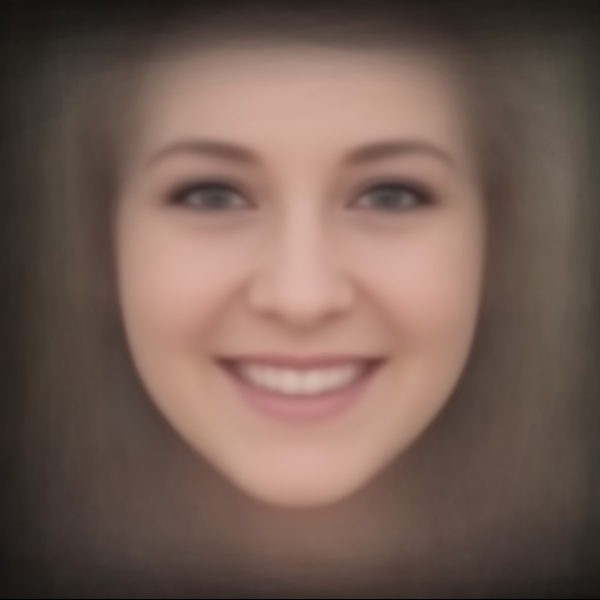
\includegraphics[width=.75\linewidth]{data/Provo_avg.jpg}
  \captionof{figure}{Average Mormon Face}
  \label{fig:avg_provo}
\end{minipage}%
\begin{minipage}{.5\textwidth}
  \centering
  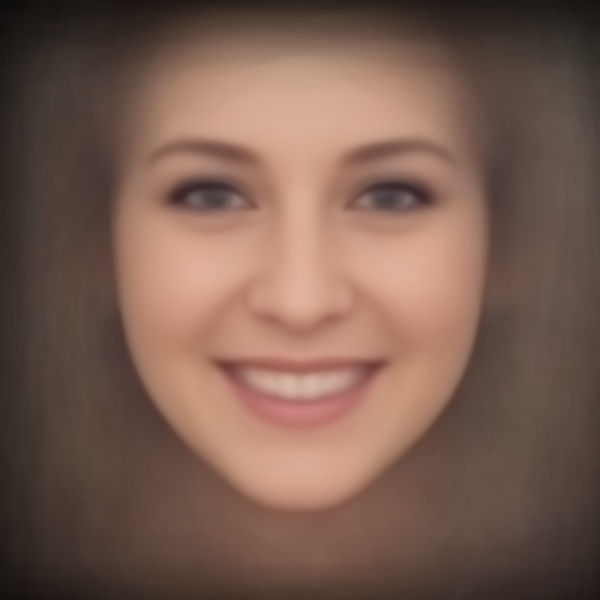
\includegraphics[width=.75\linewidth]{data/Seattle_avg.jpg}
  \captionof{figure}{Average Non-Mormon Face}
  \label{fig:avg_non}
\end{minipage}
\end{figure}

These average faces were obtained by averaging all of the pixels by the number of images in each group and then overlaying them one by one. As can be seen in the figures, there are slight differences between the two, but the difference themselves will be explored in the section on Clustering, as they're irrelevant for this algorithm. The algorithm is essentially Principal Component Analysis with the matrix being the images. 

\begin{figure}
  \centering
  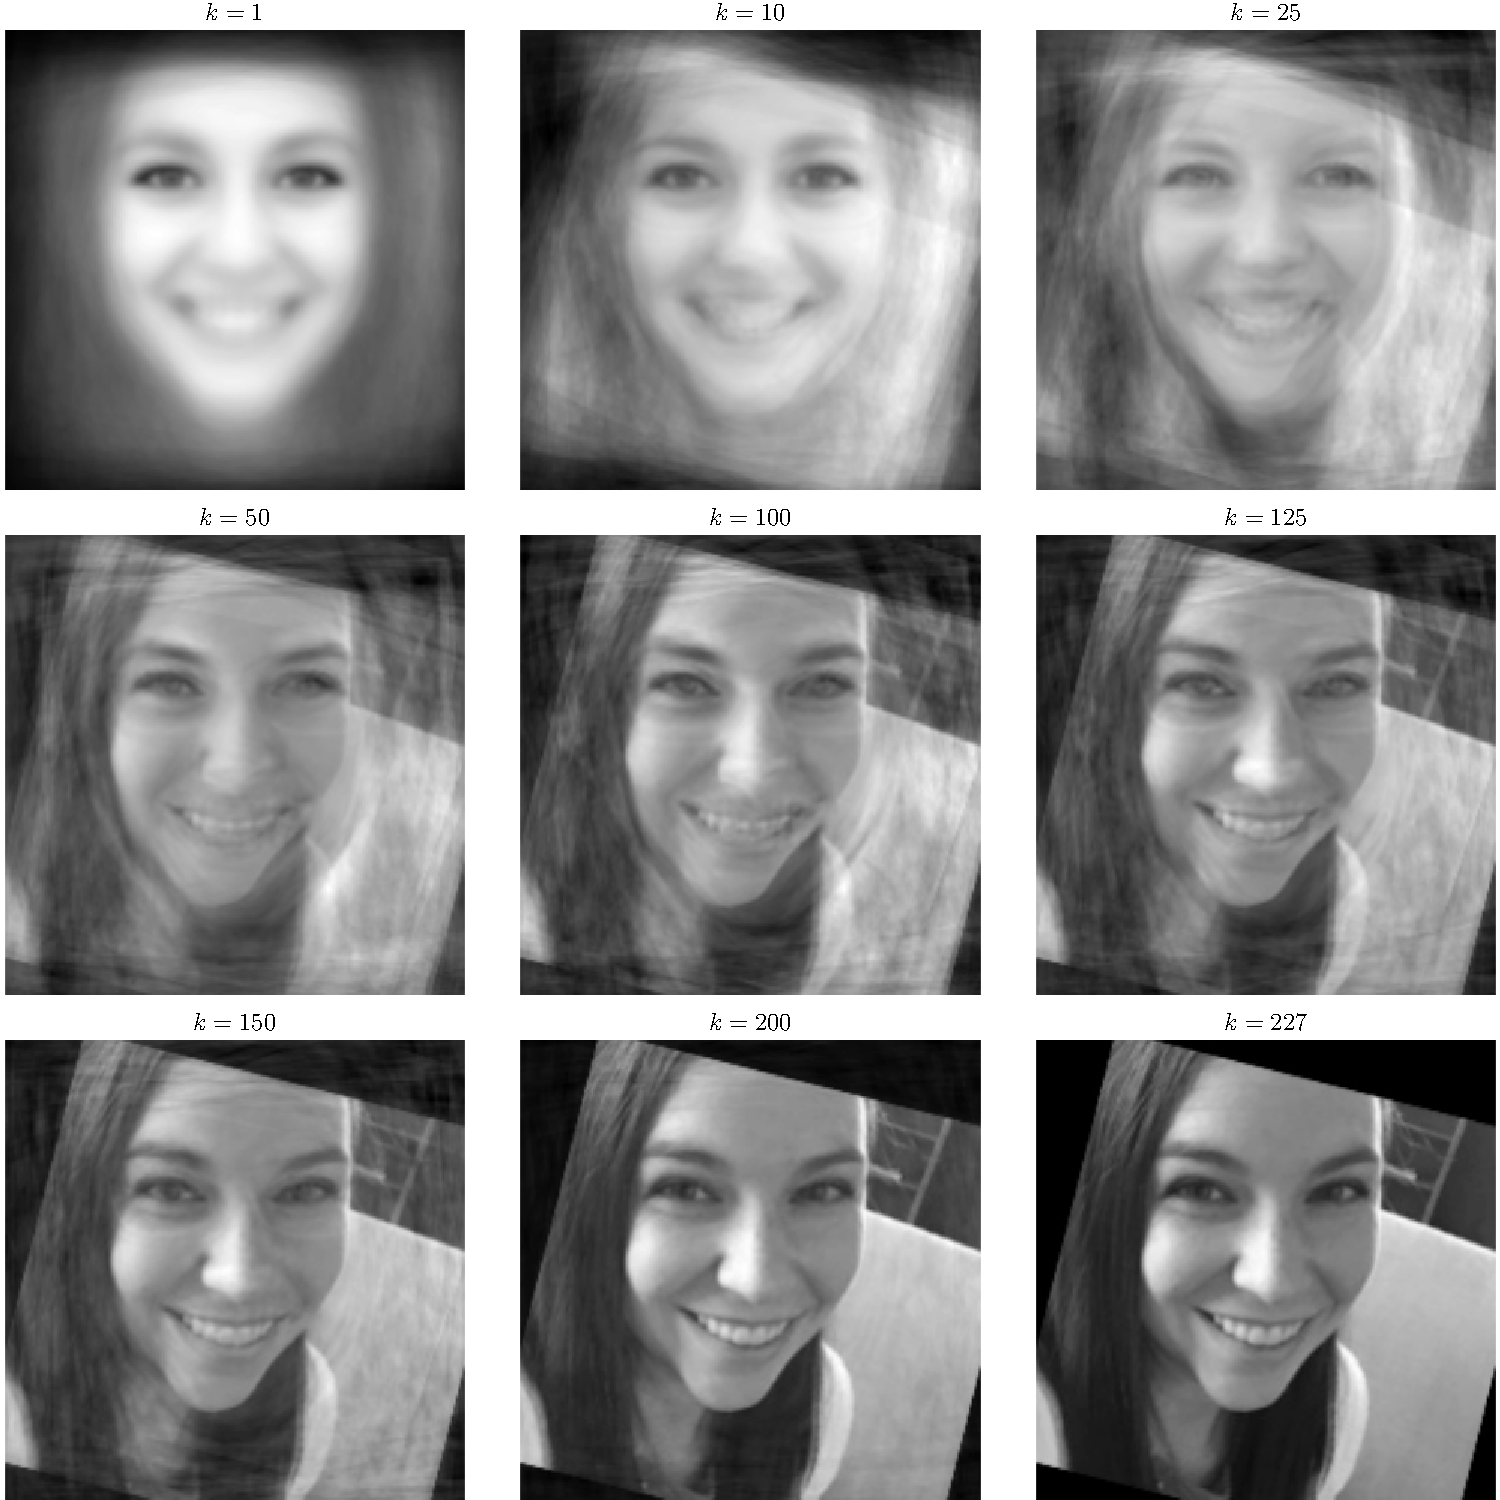
\includegraphics[width=.65\textwidth]{data/Face_Reconstruct.pdf}
  \caption{Reconstruction of a face with various values of $k$}
  \label{fig:recon}
\end{figure}

After subtracting the averages, Singlar Value Decomposition (SVD) can be performed to extract the top $k$ features. In order to determine the top features to be extracted, we can look at the variance of the singular values. The variances can be seen in Figure~\ref{fig:lam_var}, which shows the elbow occurs at around 25, which is a good indicator as a value of $k$. 

\begin{figure}
\centering
\begin{minipage}{.5\textwidth}
  \centering
  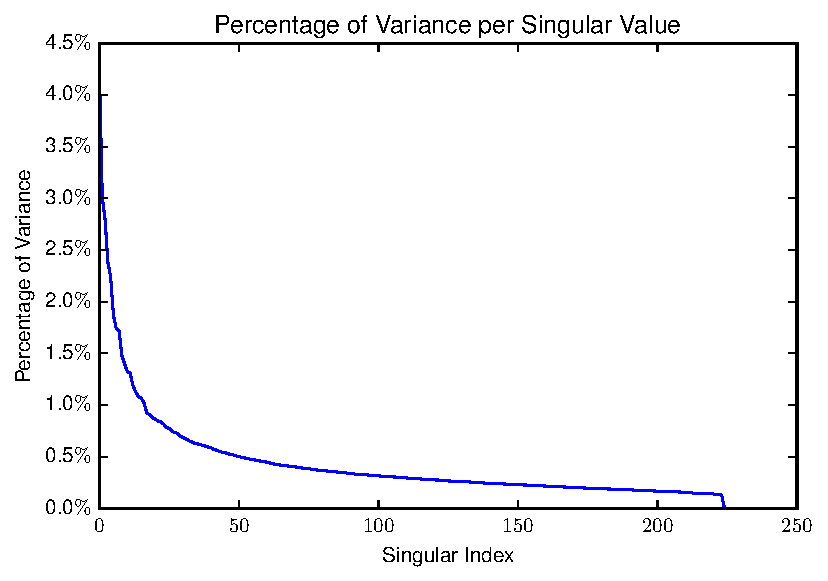
\includegraphics[width=.85\linewidth]{data/Singularvalue_Variance.pdf}
  \captionof{figure}{Variance of Singular Values from SVD}
  \label{fig:lam_var}
\end{minipage}%
\begin{minipage}{.5\textwidth}
  \centering
  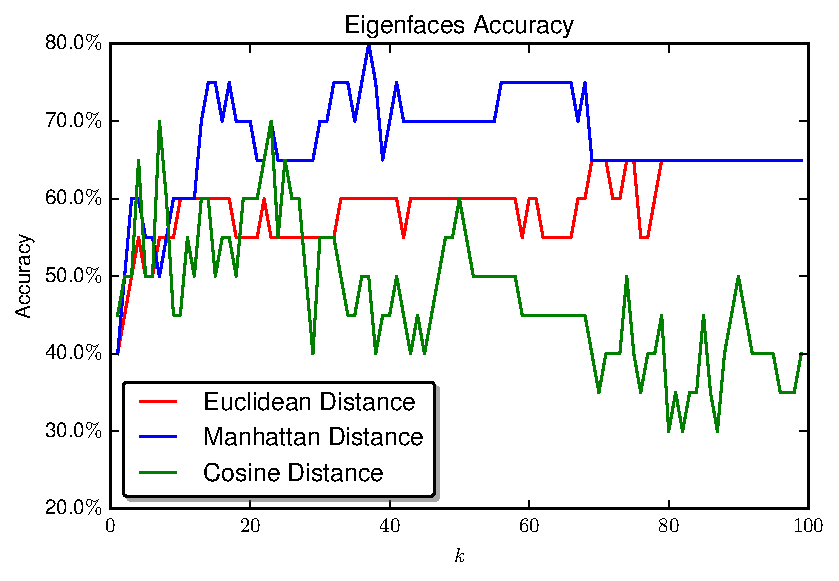
\includegraphics[width=.85\linewidth]{data/Accuracy.pdf}
  \captionof{figure}{Accuracy of Eigenfaces with various metrics}
  \label{fig:eig_acc}
\end{minipage}
\end{figure}

This variance shows that the most important features are represented with a small value of $k$, relative to the entire features of $250$. We can test over an unseen data set to see how the accuracy compares for various values of $k$, which can be seen in Figure~\ref{fig:eig_acc}. Note that the best accuracy comes about for the range $25 \leq k \leq 40$.

\section*{Clustering}

With clustering, we cannot cluster the images directly, but we can cluster SIFT features contained in the images \cite{SIFT}. SIFT features are automatically detected features in the data. In fact, we can generate SIFT features on the average faces in Figures \ref{fig:avg_provo} and \ref{fig:avg_non} to gain some insight on how to build our clustering models. These SIFT features can be seen in Figure~\ref{fig:sift_avg}. In this figure, each point represents 2 SIFT features in the above average images. It's important to note that there are large variances around the mouth and the nose between the two.

We can use the fact that there are these large difference to reduce the dimensionality. Instead of having 128 feature vectors, we can just reduce it down to the points that vary for the average images. On top of this, instead of looking at the $x$ and $y$ points, it's easy to see in Figure~\ref{fig:sift_avg} that the $x$ positions are essentially the same, and there's only a variance in the $y$, so we can drop the $x$ values as well and just focus on the prominent $y$ coordinates as the features.

\subsubsection*{Hierarchical Clustering}

For Hierarchical Clustering, as the points are relatively close, we opted to use complete-link along with the euclidean distance. Complete-Link is useful when two groups are close together in order to separate them apart. The dendrogram of the final result can be seen in Figure~\ref{fig:dendro}. The percentage of labeling accuracy that this achieved is 58.4\%. 

\begin{figure}
\centering
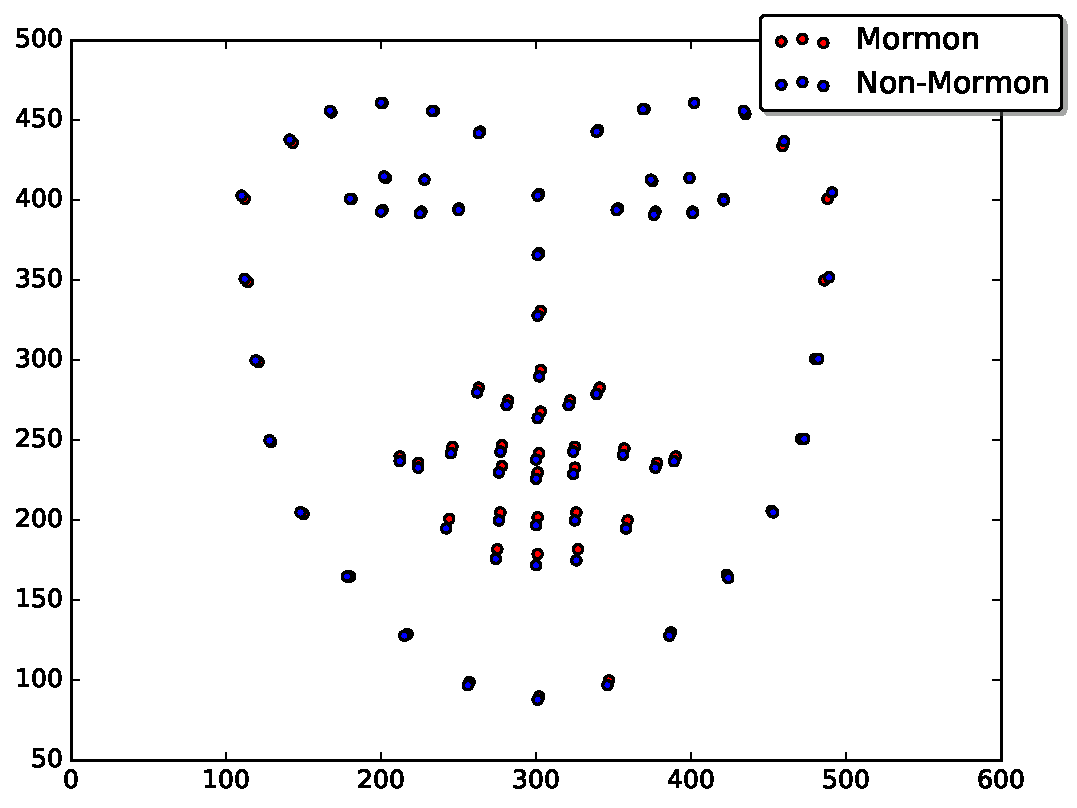
\includegraphics[width=.65\linewidth]{data/average_sift.pdf}
\caption{Average SIFT features for mormon and non-mormon}
\label{fig:sift_avg}
\end{figure}

\subsubsection*{KMeans}

As KMeans is not a deterministic algorithm, it has to be ran multiple times. Therefore, the results of the labels can be seen in Figure~\ref{fig:kmeans_cdf}. The best accuracy that was achieved was 59.3\%. 

After running KMeans, the accuracy of the labeling can be seen in Figure~\ref{fig:kmeans_label}. This figure was achieved in the following way, where $X$ is the points.

\begin{align*}
  U, \Sigma, V^{T} &= {\tt SVD}(X)\\
  U^{\dagger} &= U\cdot \Sigma
\end{align*}

From here we can take the column corresponding to the largest eigenvalue and eigenvector in $U^{\dagger}$ to get the prominent values. These are the values that are plotted in the histogram. In the top figure, those labels are from the KMeans algorithm, while the bottom figure is from the true labels. As can be seen, the labels are quite accurate and work on splitting up the data even though there isn't such a ``clean separation.''

\section*{Conclusion}

In conclusion, the unsupervised algorithms such as hierarchical clustering and KMeans did better than humans in \cite{MormonID}, with hierarchical clustering obtaining 58.4\% accuracy and KMeans 59.3\%. 

The Eigenfaces algorithm performed much better with various values of $k$ and the metric. The best metric was the Manhattan Distance which was able to achieve up to 80\% labeling accuracy for $k \sim 35$. On average, the manhattan distance performed much better than either of the aforementioned clustering algorithms. 

\section*{Group Feedback}

In meeting with another group, the feedback they gave was to try to use different distance metrics as the data is so close, and also figure out a way to reduce the dimensionality. Various metrics and agglomeration link-types were chosen for the Hierarchial Clustering case, where the best was chosen, and for KMeans and Eigenfaces multiple metrics were used. Also, the dimensionality was able to be reduced from 128 dimensions to 13, which greatly helped with the performance and the accuracy. So the feedback was useful.

\begin{figure}
\centering
\begin{minipage}{.5\textwidth}
  \centering
  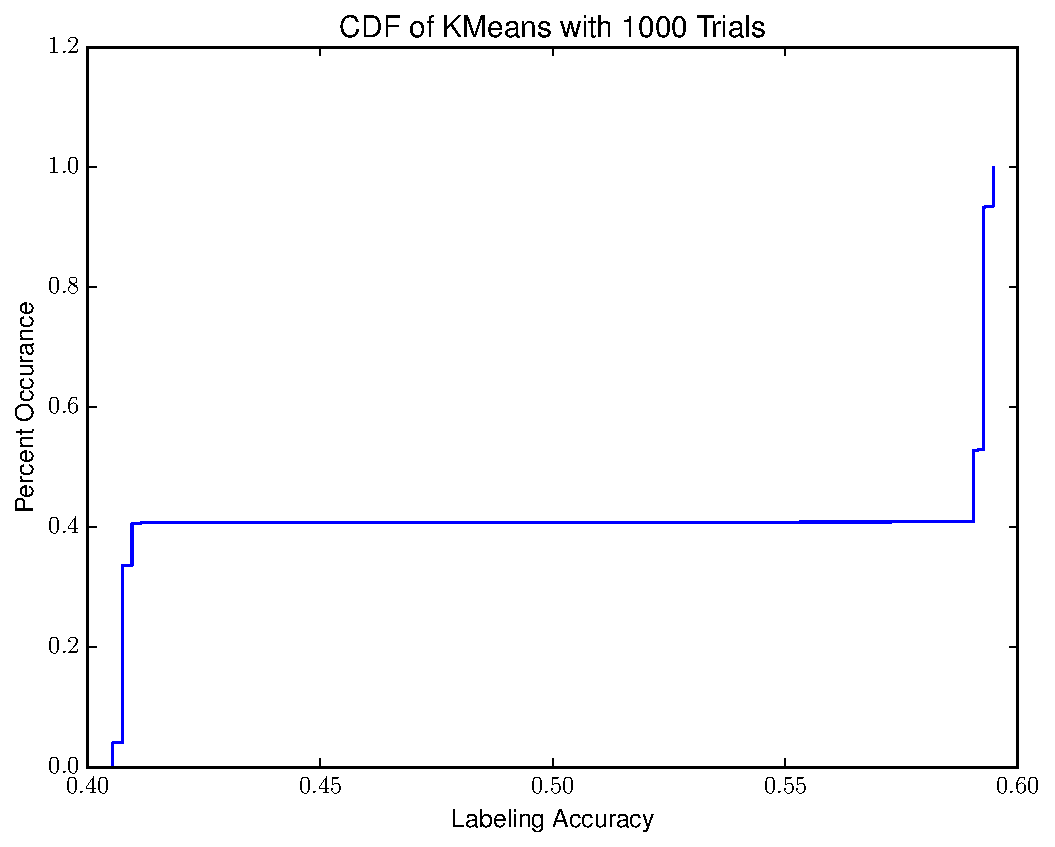
\includegraphics[width=.75\linewidth]{data/kmeans_cdf}
  \captionof{figure}{KMeans Cumulative Density Function}
  \label{fig:kmeans_cdf}
\end{minipage}%
\begin{minipage}{.5\textwidth}
  \centering
  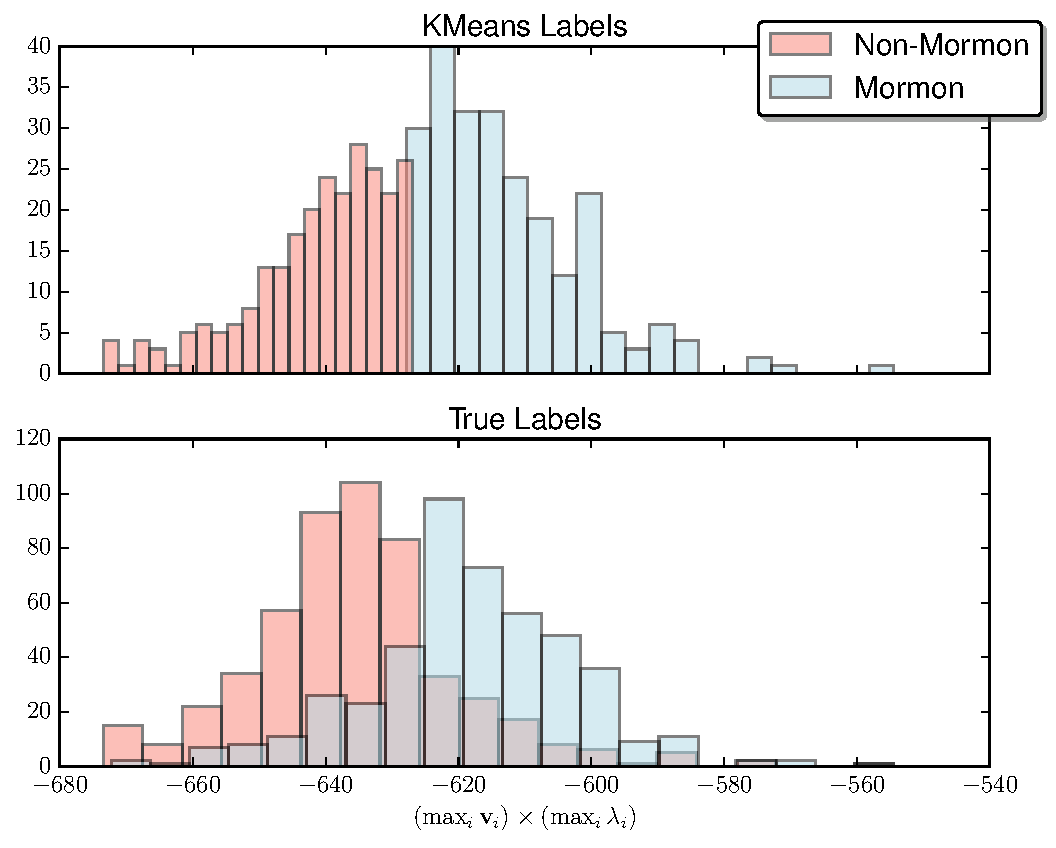
\includegraphics[width=.75\linewidth]{data/eigennorm.pdf}
  \captionof{figure}{Labeling based on largest eigenvector and eigenvalue}
  \label{fig:kmeans_label}
\end{minipage}
\end{figure}

\afterpage{\clearpage}
\begin{figure}[p]
\centering
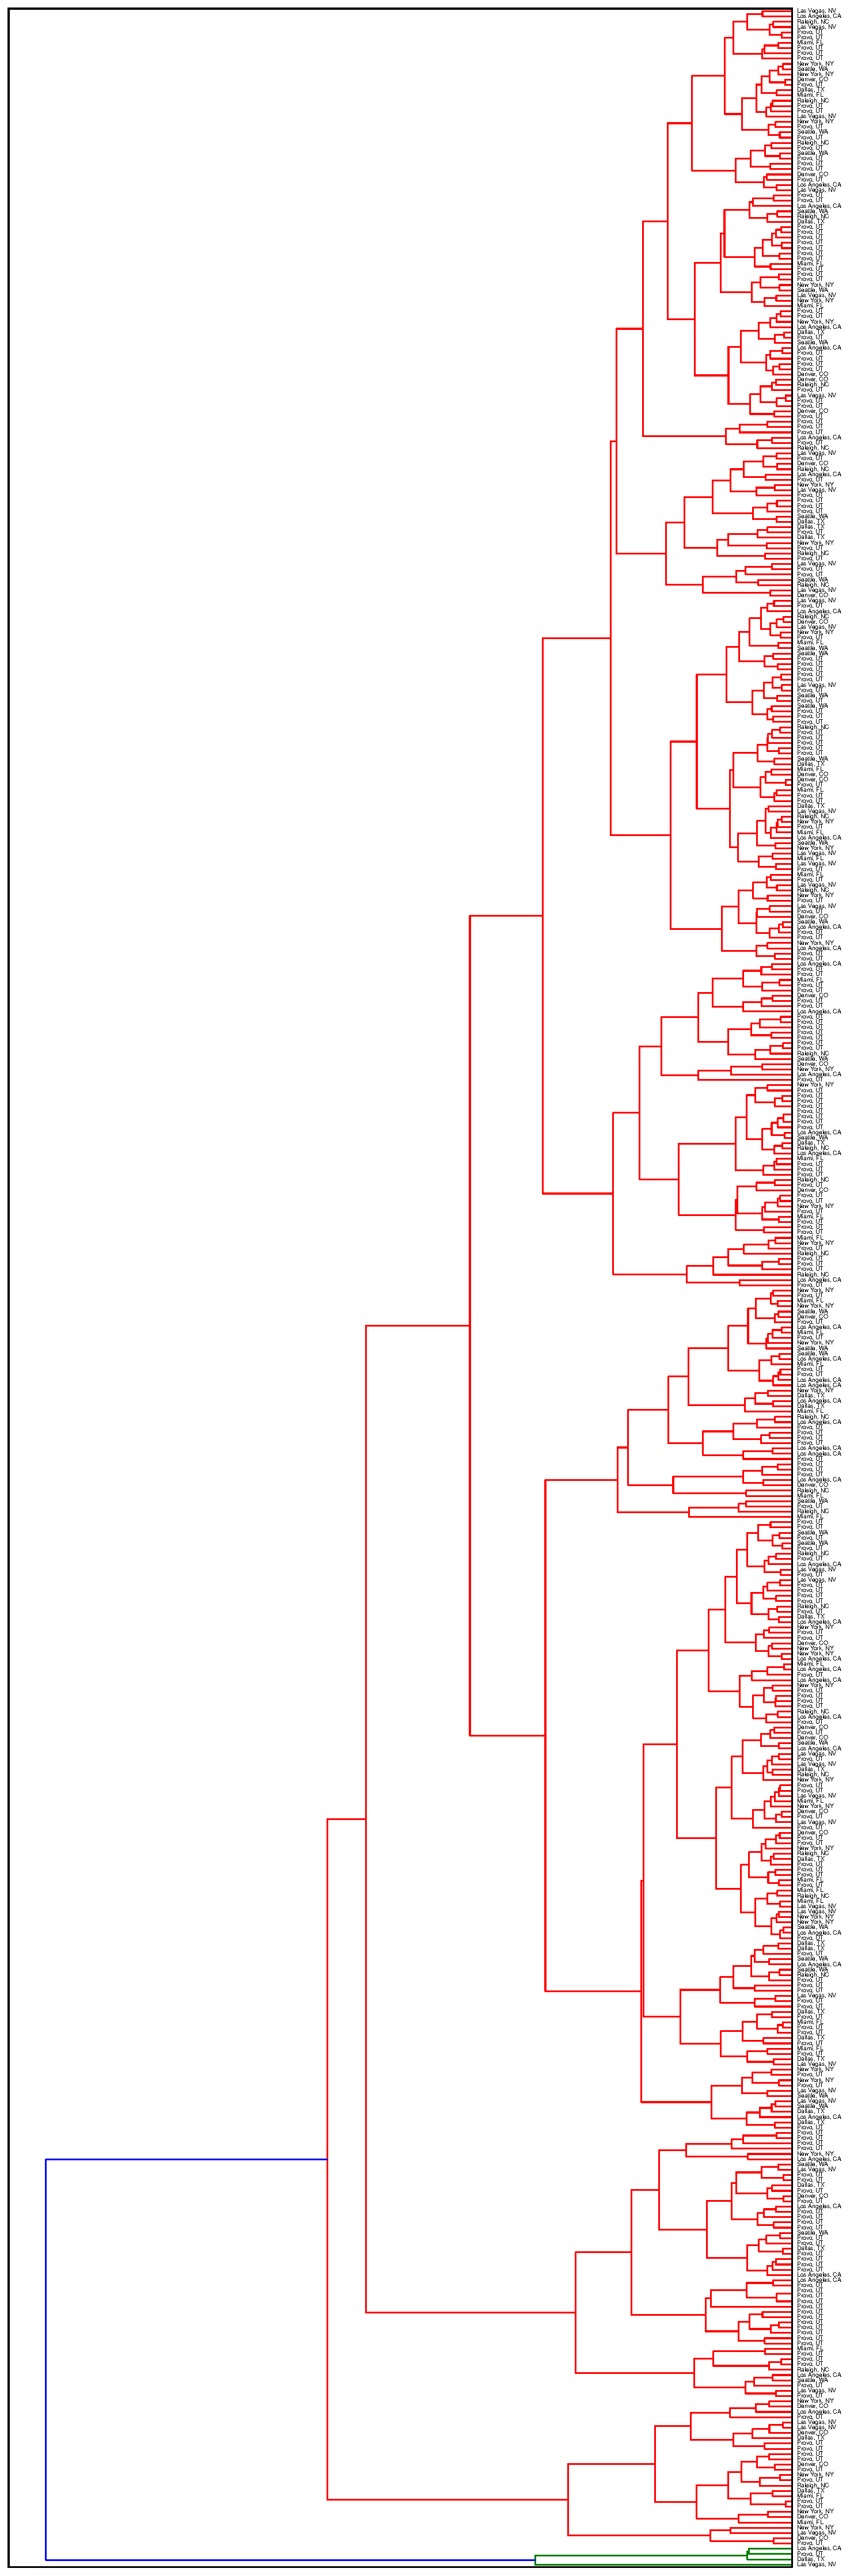
\includegraphics[height=\textheight,width=\textwidth,keepaspectratio]{data/dendrogram.pdf}
\caption{Dendrogram for Hierarchical Clustering}
\label{fig:dendro}
\end{figure}

\newpage

\bibliographystyle{plain}
\bibliography{bibliography}

\end{document}
